\chapter{Конструкторская часть}

В данном разделе сосредоточимся на создании близких к реальности приближений трехмерных объектов. 
Рассмотрим методы преобразования в трехмерном пространстве, предоставим требования к работе программы, диаграмму классов и схемы алгоритмов, которые разрабатываем.

\section{Требования к работе программы}

Программа должна обеспечить созданию реалистичных изображений. 
Важно, чтобы пользователь мог легко добавлять объекты в сцену и изменять их характеристики, такие как положение в пространстве, поверхностные свойства и спектральные характеристики, без замедлений. 

Для этого программа должна поддерживать два режима работы. 
В первом режиме акцент сделан на оперативности, чтобы пользователь мог быстро взаимодействовать с объектами.  
Во втором режиме уделяется внимание созданию реалистичных изображений.

\section{Аппроксимация трёхмерных объектов}

В рамках данной программы создадим икосферу, которая представляет собой геометрическое тело, состоящее из треугольных граней~\cite{icosphere}. Преимущество использования икосферы заключается в ее изотропии, что означает, что ее характеристики сохраняются по всем направлениям одинаково. 
Более того, распределение треугольных граней на икосфере будет более равномерным по сравнению с другими методами разбиения, что предотвратит появление артефактов и особенностей в районе полюсов сферы. Поэтому алгоритм работы программы будет следующим:
\begin{itemize}
	\item Исходя из данных о сфере, создать регулярный икосаэдр, который включает в себя 20 граней и 30 рёбер.
	\item Этот процесс повторяется до тех пор, пока не достигнута желаемая степень приближения.
\end{itemize}

На рисунке~\ref{fig:picture_1} представлен процесс пошагового приближения икосаэдра~\cite{sphere} к сфере:
\begin{figure}[h]
	\begin{center}
		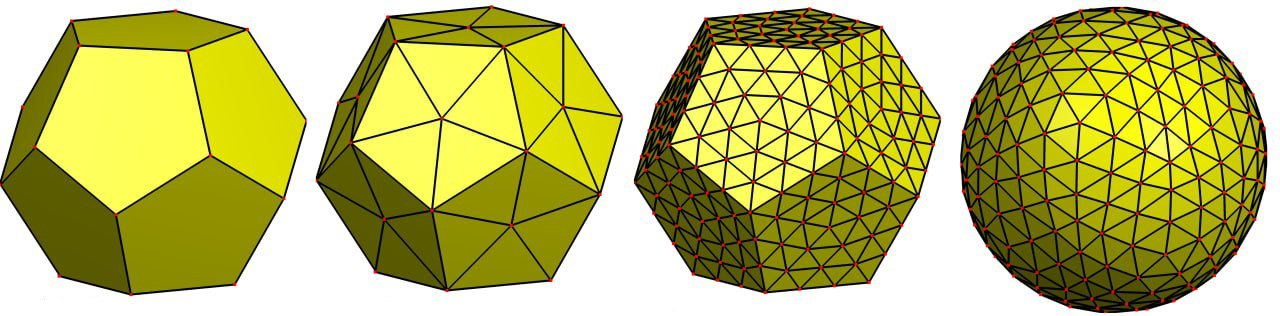
\includegraphics[width=\linewidth]{photos/sphere.png}
	\end{center}
	\caption{Процесс пошагового приближения икосаэдра к сфере}
	\label{fig:picture_1}
\end{figure}

Для корректной генерации икосаэдра важно учитывать коррекцию при вычислении координат средней точки треугольника, обозначенной как $(x_0, y_0,$ $z_0)$. 
Эта коррекция выполняется согласно формуле~\ref{fig:equation_3}:
\begin{equation}
	\begin{aligned}
		& l = \sqrt{x_0^2 + y_0^2 + z_0^2}; & x_1 = \frac{x_0}{l}; \\ 
		& y_1 = \frac{y_0}{l}; & z_1 = \frac{z_0}{l}.
	\end{aligned}
	\label{fig:equation_3}
\end{equation}

\section{Описание трёхмерных преобразований}
\subsection{Способ хранения декартовых координат}

Для представления координат точек будет использоваться вектор, состоящий из четырёх компонентов: $ x $, $y $, $z$, $w$, где $w$ по умолчанию равен 1. 
Это позволяет удобно выполнять умножение векторов на матрицы трансформации, которые имеют размерность 4x4.

\subsection{Преобразование трёхмерных координат в двухмерное пространство экрана}

Экран имеет только две координаты, поэтому необходимо разработать метод для отображения трехмерных объектов в двумерном пространстве экрана. 
Каждый пиксель на экране имеет свой цвет, и поэтому требуется найти способ передачи объема и реализма в изображении. 
Алгоритм преобразования координат включает следующие этапы:
\begin{itemize}
	\item преобразовать объект из его собственного пространства в мировое пространство;
	\item перевести объект из мирового пространства в пространство камеры;
	\item найти проекции всех точек из пространства камеры на видимые точки, где координаты $x$, $y$ и $z$ находятся в диапазоне от $-w$ до $w$, а $w$ находится в диапазоне от 0 до 1;
	\item масштабировать все точки, полученные на шаге 3, для отображения на экране с требуемым разрешением.
\end{itemize}

Для выполнения всех этих преобразований необходимо применять матрицы преобразований. 
Сначала рассчитываются все необходимые матрицы, а затем они перемножаются в заданном порядке. 
Исходные координаты умножаются на конечный результат, что приводит к преобразованию координат в нужную систему.

\subsection{Преобразования трёхмерной сцены в пространство камеры}

Для приведения трехмерной сцены в пространство камеры необходимо умножить каждую вершину всех полигональных моделей на матрицу камеры. 
Камера сама по себе задается несколькими параметрами: положением в мировом пространстве, вектором направления взгляда и направлением верха камеры. Пусть:
\begin{itemize}
	\item $\alpha$ -- это координаты точки, на которую камера смотрит;
	\item $\beta$ -- вектор, указывающий, куда направлена верхняя часть камеры;
	\item $\gamma$ --  вектор, ортогональный векторам направления взгляда и верхнему направлению.
\end{itemize}
Таким образом, матрица камеры будет иметь следующий вид:
\begin{equation}
	B = \left(
	\begin{array}{cccc}
		\alpha_x & \beta_x & \gamma_x & 0\\
		\alpha_y & \beta_y & \gamma_y & 0 \\
		\alpha_z & \beta_z & \gamma_z & 0 \\
		-(P*\alpha) & -(P*\beta) &-(P*\gamma) & 1
	\end{array}
	\right) 
\end{equation}

\subsection{Матрица перспективной проекции}

После перехода в камерное пространство, каждая вершина полигональных моделей подвергается умножению на матрицу проекции. 
Эта матрица изменяет усеченную пирамиду видимости в пространство отсечения и регулирует значение $w$-компоненты. 
При этом, чем дальше вершина находится от наблюдателя, тем больше становится значение $w$. 
После проецирования координат, значения $x$ и $y$ находятся в интервале от $-w$ до $w$, а $z$ находится в интервале от $0$ до $w$. 
Все объекты, которые находятся за пределами этого диапазона, будут отсечены.

Пусть:
\begin{itemize}
	\item B -- это отношение ширины изображения к его высоте;
	\item $\phi$ -- угол обзора камеры;
	\item Zb -- координата z ближайшей к камере плоскости отсечения в пирамиде видимости;
	\item Ze -- координата z дальней от камеры плоскости отсечения в пирамиде видимости.
\end{itemize}

Тогда матрица перспективной проекции будет будет представлять собой:
\begin{equation}
	A = \left(
	\begin{array}{cccc}
		\frac{cot(\frac{\phi}{2})}{B} & 0 & 0 & 0\\
		0 & cot(\frac{\phi}{2}) & 0 & 0 \\
		0 & 0 & \frac{Z_e \times Z_b}{Z_e - Z_b} & 1 \\
		0) & 0 & \frac{Z_e}{Z_e - Z_b} & 0
	\end{array}
	\right)
\end{equation}

На следующем этапе хотим проецировать все координаты на одну плоскость, путем разделения всех координат на значение $z$. 
После умножения вектора координат на матрицу перспективной проекции, реальная координата $z$ перемещается в компоненту $w$. 
Вместо деления на $z$ делим на $w$.

\subsection{Преобразования трёхмерной сцены в пространство области изображения}

Чтобы преобразовать спроецированные координаты в координаты области изображения, мы умножаем вектор координат на специальную матрицу.
Пусть:
\begin{itemize}
	\item $W$ -- ширина изображения;
	\item $H$ -- высота изображения;
	\item $hW$ -- половина ширины изображения;
	\item $hH$ -- половина высоты изображения.
\end{itemize}

Тогда матрица, которая выполняет это преобразование, будет представлять собой:
\begin{equation}
	A = \left(
	\begin{array}{cccc}
		hW & 0 & 0 & hW\\
		0 & hH & 0 & hH \\
		0 & 0 & 1 & 0 \\
		0 & 0 & 0 & 1
	\end{array}
	\right)
\end{equation}

\section{Алгоритм обратной трассировки лучей}

На схеме в рисунке~\ref{fig:raytrace} представлено, как работает алгоритм обратной трассировки лучей.
\FloatBarrier
\begin{figure}[h]
	\begin{center}
		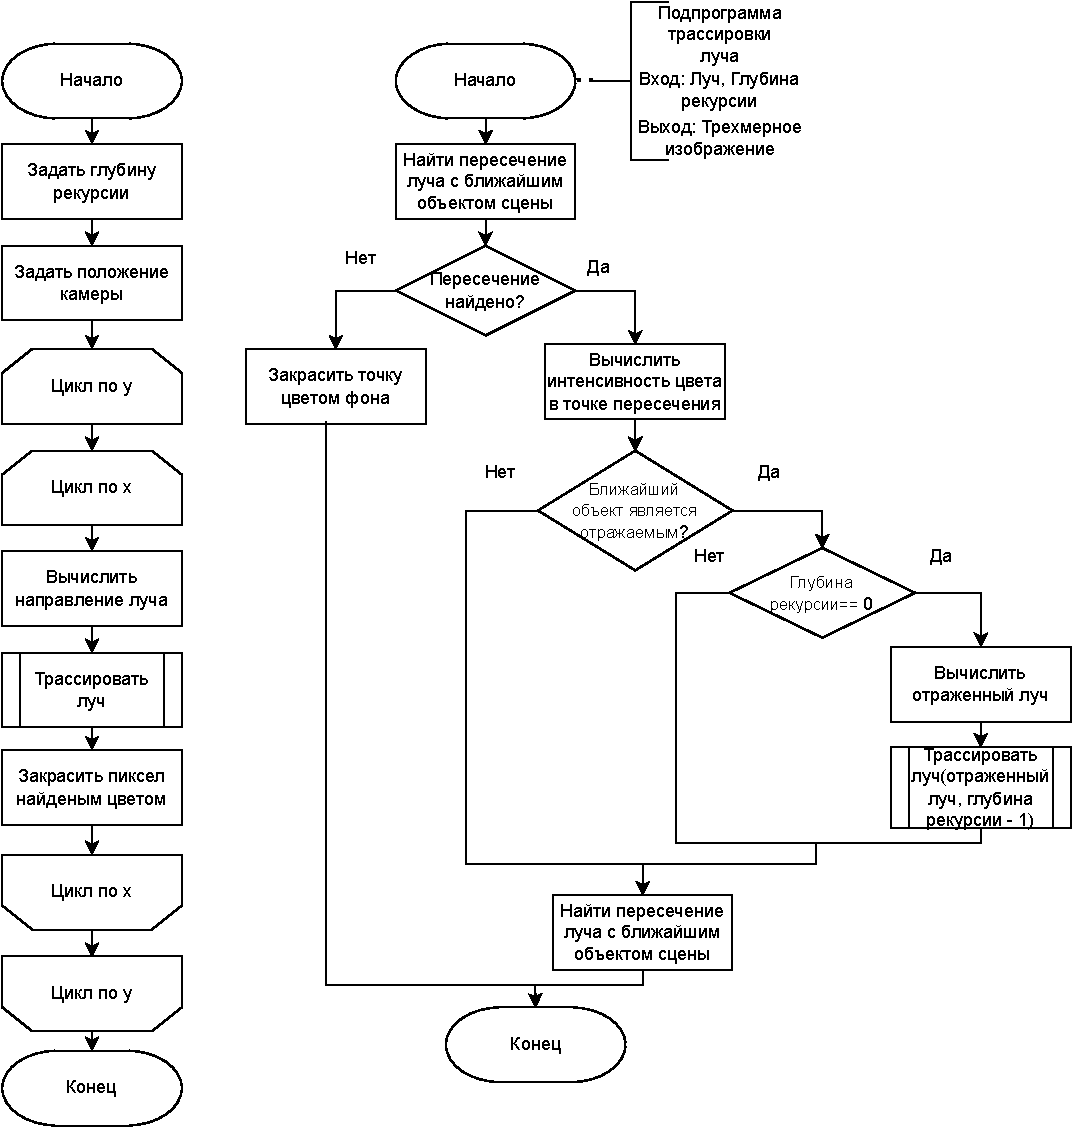
\includegraphics[width=\linewidth]{photos/ray_tracing.pdf}
	\end{center}
	\caption{Схема реализации алгоритма обратной трассировки лучей}
	\label{fig:raytrace}
\end{figure}
\FloatBarrier

На схеме в рисунке~\ref{fig:fongo} представлено, как работает алгоритм Фонга.
\FloatBarrier
\begin{figure}[h]
	\begin{center}
		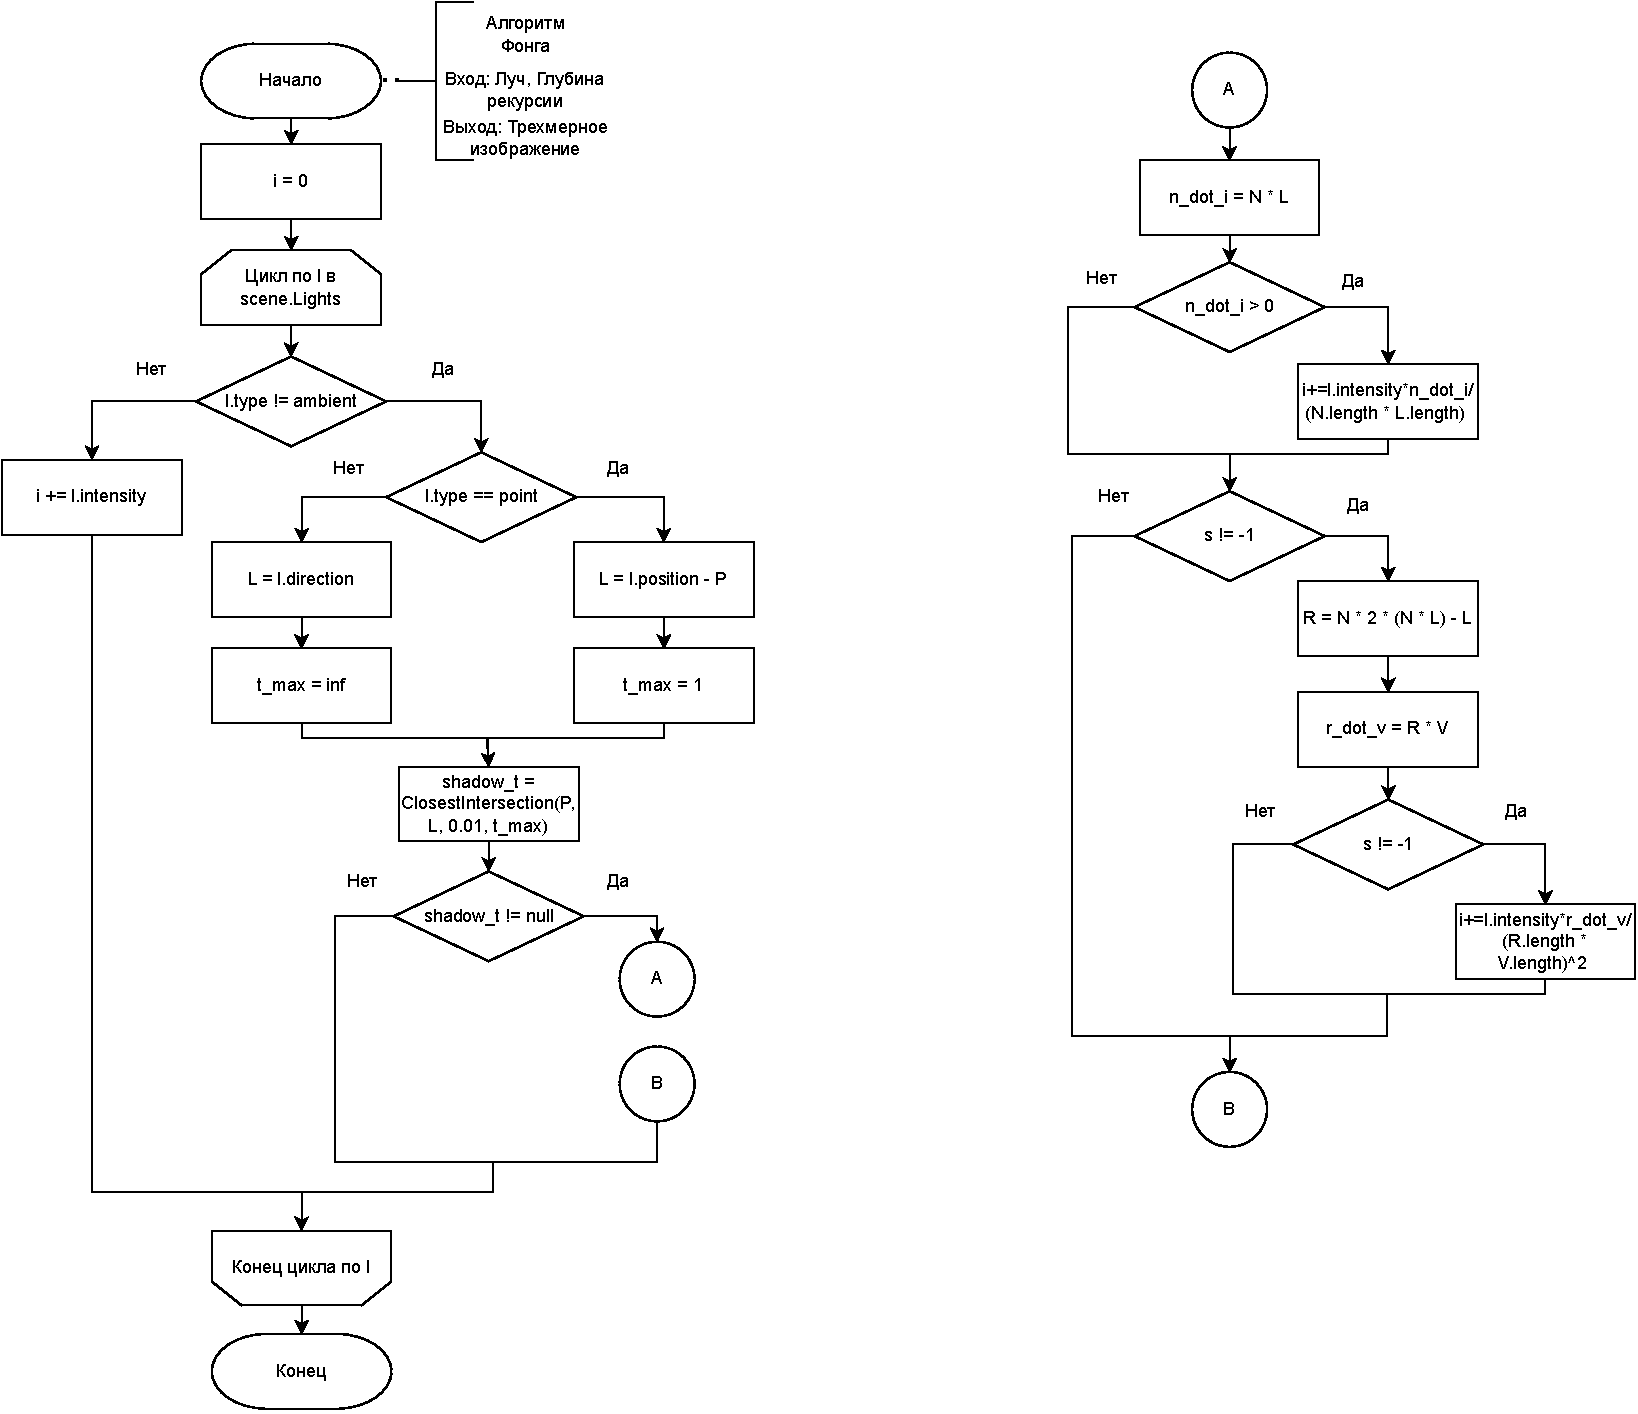
\includegraphics[width=\linewidth]{photos/fonga.pdf}
	\end{center}
	\caption{Схема реализации алгоритма Фонга}
	\label{fig:fongo}
\end{figure}
\FloatBarrier

Для эффективной реализации алгоритма обратной трассировки лучей, необходимо уметь вычислять направление отраженных и преломленных лучей, учитывая при этом модель освещения Фонга. 
Для нахождения отраженного луча, нужно знать направление падающего луча и нормаль к поверхности.

Пусть: 
\begin{itemize}
	\item $\overline{L}$ -- направление луча;
	\item $\overline{n}$ -- нормаль к поверхности. 
\end{itemize}

Луч можно разбить на две части: $\overline{L_n}$ которая перпендикулярна нормали, и  $\overline{L_n}$ – параллельна нормали.

Иллюстрация этой ситуации изображена на рисунке~\ref{fig:picture_2}:
\FloatBarrier
\begin{figure}[h]
	\begin{center}
		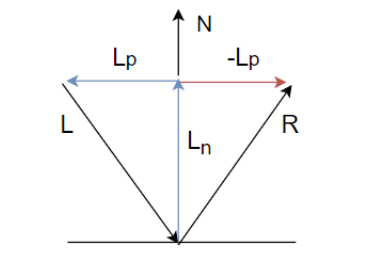
\includegraphics[]{photos/vectors.png}
	\end{center}
	\caption{Рассматриваемые векторы для расчёта отражённого луча.}
	\label{fig:picture_2}
\end{figure}
\FloatBarrier

Учитывая свойства скалярного произведения $ \overline{L_n} = \overline{n} * (\overline{n}, \overline{L}) $ и  $ \overline{L_p} = \overline{L} - \overline{n} * (\overline{n}, \overline{L}), $ так как отражённый луч выражается через разность этих векторов, то отражённый луч выражается по формуле~\ref{fig:equation_4}:
\begin{equation}
	R = 2*\overline{n}*(\overline{n}, \overline{L}) - \overline{L}.
	\label{fig:equation_4}
\end{equation}

Согласно закону преломления, луч света падающий на поверхность, луч преломлённого света и нормаль к этой поверхности лежат в одной плоскости.
Обозначим показатели преломления сред как $\mu_i$, а углы падения и отражения света как $\eta_i$. 
Применяя закон Снеллиуса, можем вычислить параметры преломлённого луча с использованием формулы~\ref{fig:equation_5}:
\begin{equation}
	\begin{aligned}
		& R = \frac{\mu_1}{\mu_2} \overline{L} + ( \frac{\mu_1}{\mu_2} cos(\eta_1) - cos(\eta_2))\overline{n}; \\ 
		& cos(\eta_2) = \sqrt{1 - (\frac{\mu_1}{\mu_2})^2 * (1 - cos(\eta_1))^2}.
	\end{aligned}
	\label{fig:equation_5}
\end{equation} 

\section{Алгоритм пересечения луча с параллелепипедом}

Для эффективного выполнения алгоритма обратной трассировки лучей, нецелесообразно искать пересечения с каждым полигоном в сцене каждый раз при трассировке луча. 
Поэтому имеет смысл ограничивать объекты в сцене параллелепипедами, которые полностью их охватывают.

Эти параллелепипеды определяются координатами двух вершин: минимальной и максимальной по значениям координат $x$, $y$ и $z$. 
Это позволяет задать шесть плоскостей, которые ограничивают параллелепипед, и все они параллельны координатным осям.

Рассмотрим пару плоскостей, которые параллельны плоскости $yz$: $X$ = $x_1$ и $X$ = $x_2$. 
Предположим, что есть вектор направления луча $\overline{D}$. 
Если $x$ -- координата вектора $\overline{D}$ равна нулю, это означает, что луч параллелен этим плоскостям. 
В таком случае, если $x_0$ (начальная $x$ -- координата луча) меньше $x_1$ или больше $x_2$, луч не пересекает рассматриваемый прямоугольный параллелепипед.

Однако, если $\overline{D_x}$ (проекция вектора $\overline{D}$ на ось $x$) не равна нулю, мы можем вычислить следующие отношения:
\begin{equation}
	\begin{aligned}
		& t_{1x} = \frac{x_1 - x_0}{\overline{D_x}}; \\ 
		& t_{2x} = \frac{x_2 - x_0}{\overline{D_x}}. \\
	\end{aligned}
\end{equation} 

Можно считать, что найденные величины связаны неравенством $t_{1x} < t_{2x}$.
Пусть $t_n = t_{1x}$, $t_f = t_{2x}$. 
Считая, что $D_y$ не равно нулю, и рассматривая вторую пару плоскостей, несущих грани заданного параллелепипеда, $Y = y_1$, $Y = y_2$, вычисляются величины:

\begin{equation}
	\begin{aligned}
		& t_{1y} = \frac{y_1 - y_0}{D_y}; \\ 
		& t_{2y} = \frac{y_2 - y_0}{D_y}. \\
	\end{aligned}
\end{equation} 

Если $t_{1y} > t_n$, то тогда $t_n = t_{1y}$.
Если $t_{2y} < t_f$, то тогда $t_f = t_{2y}$.
При $t_n > t_f$ или при $t_f < 0$ заданный луч проходит мимо прямоугольного параллелепипеда.

Считая, что $\overline{D_z}$ не равно нулю, и рассматривая вторую пару плоскостей, несущих грани заданного параллелепипеда, $Z = z_1$, $Z = z_2$, вычисляются величины:

\begin{equation}
	\begin{aligned}
		& t_{1z} = \frac{z_1 - z_0}{\overline{D_z}}; \\ 
		& t_{2z} = \frac{z_2 - z_0}{\overline{D_z}}, \\
	\end{aligned}
\end{equation} 
и повторяются сравнения, приведённые для формулы 2.6.

Если после выполнения всех операций мы получаем такие значения, что $0 < t_n < t_f$ или $ 0 < t_f$, то это означает, что исходный луч пересекает ограничивающий параллелепипед, у которого стороны параллельны координатным осям.

Важно учесть, что при внешнем пересечении лучом параллелепипеда, значения $t_n$ и $t_f$ должны быть равны. В противном случае можно заключить, что луч пересекает параллелепипед изнутри.
\clearpage

\section{Диаграмма классов}

На рисунке~\ref{fig:diagramm} представлена диаграмма классов.
\FloatBarrier
\begin{figure}[h]
	\begin{center}
		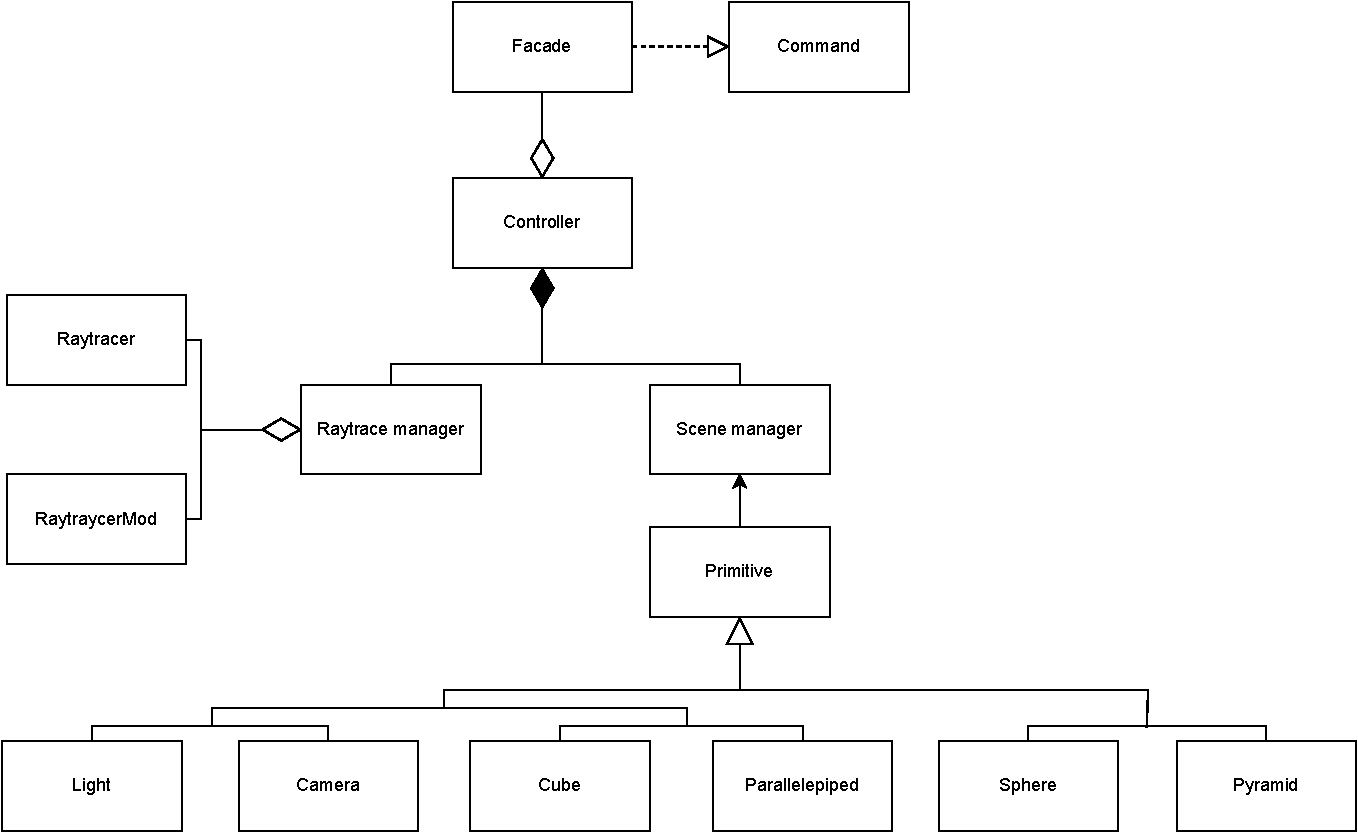
\includegraphics[width=\linewidth]{photos/diagram.pdf}
	\end{center}
	\caption{Диаграмма классов}
	\label{fig:diagramm}
\end{figure}
\FloatBarrier

Классы объектов:
\begin{itemize}
	\item Primitive -- базовый класс объектов;
	\item Sphere -- класс шара;
	\item Pyramid -- класс пирамиды;
	\item Cube -- класс куба;
	\item Parallelepiped -- класс параллелепипед;
	\item Camera -- класс камеры;
	\item Light -- класс источника света;
	\item Facade -- класс, предоставляющий интерфейс работы системы;
	\item Controller - класс, который позволяет взаимодействовать управляющие классы с классами интерфейса;
	\item Raytracer -- класс визуализации сцены.
\end{itemize}

\section{Проекция программного обеспечения}

На рисунках~\ref{fig:idef0_1} -- \ref{fig:idef0_2} представлена проекция программного обеспечения.
\begin{figure}[h]
	\begin{center}
		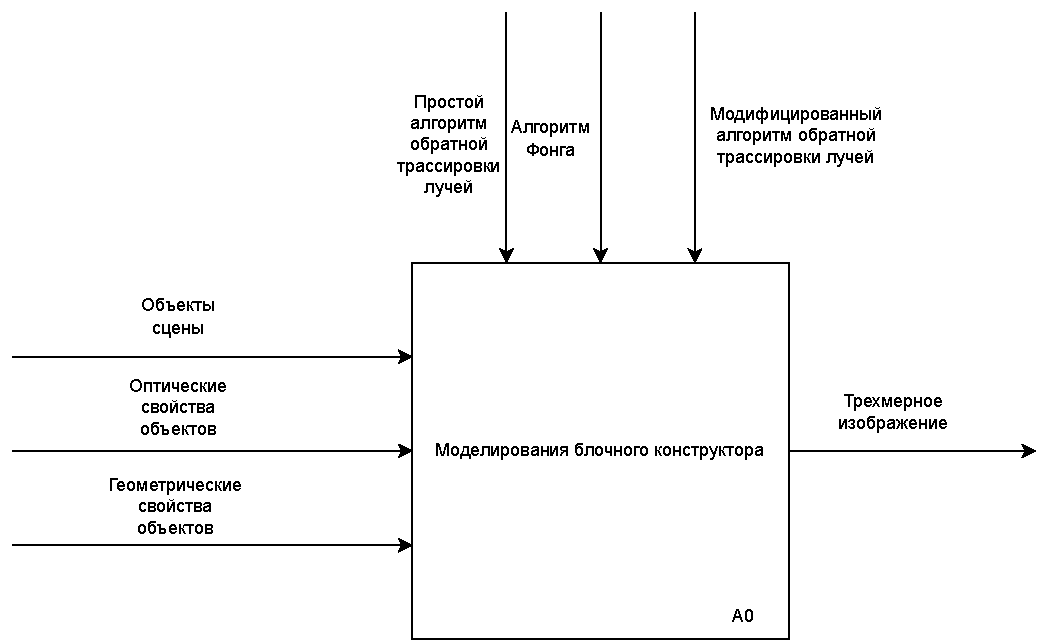
\includegraphics[width=\linewidth]{photos/idef0_1.pdf}
	\end{center}
	\caption{Проекция программного обеспечения}
	\label{fig:idef0_1}
\end{figure}
\clearpage

\begin{figure}[h]
	\begin{center}
		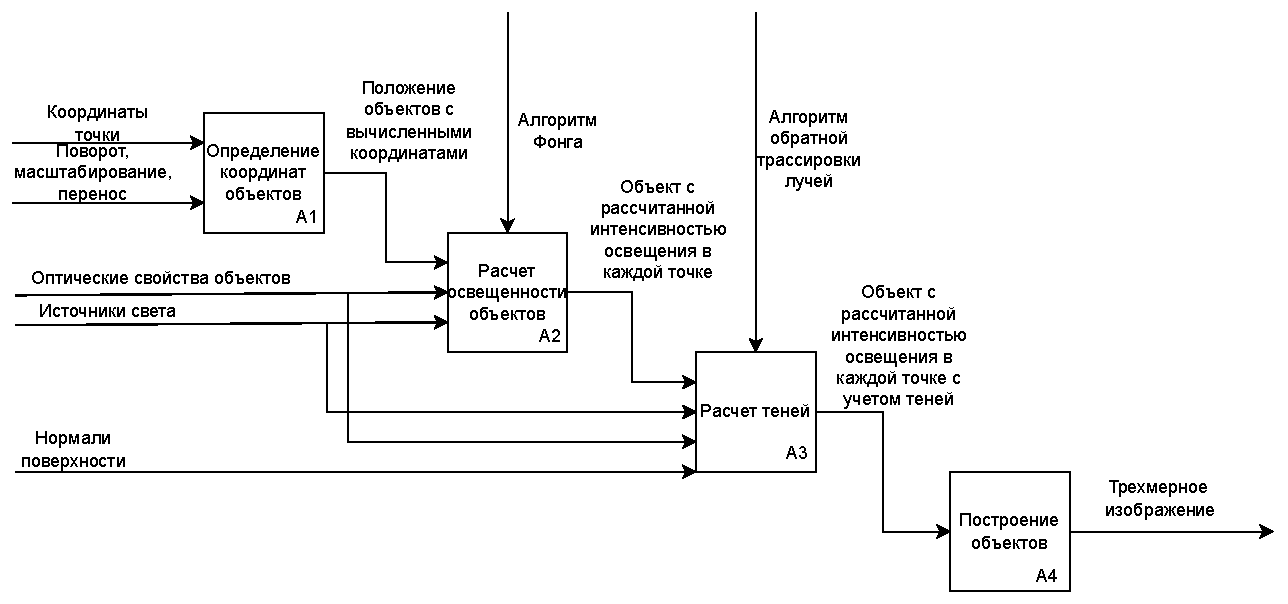
\includegraphics[width=\linewidth]{photos/idef0_2.pdf}
	\end{center}
	\caption{Проекция программного обеспечения}
	\label{fig:idef0_2}
\end{figure}

\section*{Вывод}
В данном разделе провели анализ приближения трехмерных объектов. 
Изучили трехмерные трансформации, указали требования к программному обеспечения. 
Также предоставили проекцию программного обеспечения, схему алгоритмов и  диаграмму классов.